\section{等度连续性}
\label{sec:mmap-equicontinuity}

上一节研究的是一列映射趋于一个极限；有时我们关心的是一整族映射作为整体有多“规整”。例如一族函数各自连续，但随着下标增大越来越陡，它们在同一个输入点附近需要的阈值就越来越小。

均匀连续说的是$\delta$与位置无关，等度连续把这个想法换成$\delta$与族中的成员无关。本节给出定义，并证明在紧定义域上，两种“无关”可以同时实现。

\paragraph{等度连续的定义}
在$[0,1]$上看映射族$\mathcal F=\{x^n:n\geq1\}$，每个$x^n$都连续。先看$x_0=1$，取$\varepsilon=1/2$。对任何$\delta\in(0,1)$，令$x=1-\delta/2$，则$\lvert x-1\rvert<\delta$，而$(1-\delta/2)^n\to0$，所以$n$充分大时
\[
 \lvert x^n-1^n\rvert>\frac12.
\]
没有一个$\delta$对全族有效。

在$x_0=1/2$处情况不同，这里可以把全族分成两组来处理。取$\varepsilon=1/10$，先限制$\lvert x-1/2\rvert<1/4$，此时$x<3/4$，于是
\[
 \lvert x^n-(1/2)^n\rvert\leq(3/4)^n.
\]
由$(3/4)^9\approx0.075$，$n\geq9$的成员在这个半径上已经满足要求。

剩下$n=1,\ldots,8$这八个成员，用中值定理估计。对$x,x'\in[0,3/4]$，
\[
 \lvert x^n-x'^n\rvert\leq n(3/4)^{n-1}\lvert x-x'\rvert\leq\frac{27}{16}\lvert x-x'\rvert,
\]
这里系数$n(3/4)^{n-1}$在$n=3,4$处取最大值$27/16=1.6875$。

要使右端小于$1/10$，只需$\lvert x-x'\rvert<8/135$，于是全族共用的半径可以取
\[
 \delta=\frac1{17}.
\]
验算：$1/17<8/135$，并且$1/17<1/4$，所以这个$\delta$对全部$n$都有效。

\begin{definition}[等度连续]
\label{def:mmap-equicontinuous}
设$\mathcal F$是一族映射$X\to Y$，$x\in X$。若对任意$\varepsilon>0$，存在$\delta>0$，使得对所有$f\in\mathcal F$和所有$x'\in X$，
\begin{equation}
 d(x,x')<\delta
 \quad\Longrightarrow\quad
 d(f(x),f(x'))<\varepsilon,
 \label{eq:mmap-equicontinuous}
\end{equation}
则称$\mathcal F$在$x$处\term{等度连续}（equicontinuous）。若$\mathcal F$在$X$的每一点等度连续，称$\mathcal F$在$X$上等度连续。若$\delta$还可以对所有$x$通用，称$\mathcal F$\term{一致等度连续}（uniformly equicontinuous）。
\end{definition}

上面的$\{x^n\}$在每个$x_0\in[0,1)$处等度连续：取$\delta_0=(1-x_0)/2$，$B(x_0,\delta_0)$内的点都不超过$r=(1+x_0)/2<1$，$r^n$最终小于$\varepsilon$，前面有限个成员再各取一个半径，与$\delta_0$取最小值即可。在$x_0=1$处不等度连续。

每个成员连续，只说明每个$f$都有自己的$\delta_f$；等度连续要求这些$\delta_f$有正的下界。有限族总是满足这一点，取有限个$\delta_f$的最小值就行；无限族则可能不满足，下面的例子把两种情形并排放在一起。

\paragraph{等度连续的例子}
共同的Lipschitz常数给出最简单的等度连续族。若每个$f\in\mathcal F$都满足$d(f(x),f(x'))\leq Ld(x,x')$，取$\delta=\varepsilon/L$，它对所有成员和所有点都有效，所以族一致等度连续。例如平移族$\{x\mapsto\sin(x+c):c\in\mathbb R\}$，每个成员的导数绝对值不超过$1$，是$1$-Lipschitz族。

频率不断增大的族则不然。$\{x\mapsto\sin(nx):n\geq1\}$在$0$处不等度连续：对任何$\delta>0$，取$n>\pi/(2\delta)$，点$x'=\pi/(2n)$满足$\lvert x'\rvert<\delta$，而
\[
 \lvert\sin(nx')-\sin0\rvert=1.
\]

图~\ref{fig:mmap-equicontinuity}并排画出这两族。左边的曲线在宽度$\delta$的窗口内一起缓慢变化，右边的曲线随$n$增大越来越早地冲到$1$，无论窗口多窄，总有成员在窗口内完成一次满振幅。

\begin{BookInlineFigure}
  \centering
  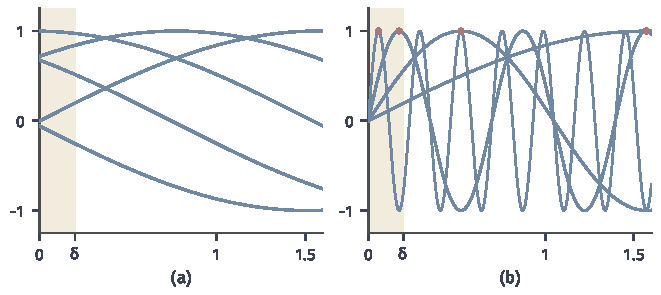
\includegraphics[width=112mm]{figures/04-spaces-measures-and-geometry/01-topology-and-metric/matplotlib/mmap-equicontinuity/figure.pdf}
  \caption{等度连续与不等度连续。(a) 平移族$\sin(x+c)$，$c=0,0.8,1.6,2.4,3.2$，导数绝对值不超过$1$，在宽度$\delta=0.2$的窗口（黄色）内每条曲线的变化不超过$0.2$。(b) $\sin(nx)$，$n=1,3,9,27$，红点是首次到达$1$的位置$x=\pi/(2n)$，当$n$足够大时落进任何给定的窗口。}
  \label{fig:mmap-equicontinuity}
\end{BookInlineFigure}

\paragraph{紧定义域上的统一半径}
均匀连续与连续之间的关系，对映射族同样成立：在紧定义域上，逐点的等度连续可以升级为一致的等度连续。

\begin{theorem}[紧空间上的一致等度连续]
\label{thm:mmap-compact-uniform-equicontinuous}
设$X$是紧致度量空间，$\mathcal F$是在$X$上等度连续的映射族。则$\mathcal F$一致等度连续。
\end{theorem}

\begin{proof}
反证。若结论不成立，存在$\varepsilon>0$，以及$f_n\in\mathcal F$和点列$x_n,x_n'$，使
\[
 d(x_n,x_n')<\frac1n,\qquad d(f_n(x_n),f_n(x_n'))\geq\varepsilon.
\]

由序列紧致性，取子列$x_{n_k}\to x\in X$，由三角不等式，$x'_{n_k}$也趋于$x$。在$x$处用等度连续，取对应于$\varepsilon/2$的$\delta$。

当$k$充分大时，$x_{n_k}$与$x'_{n_k}$都落在$B(x,\delta)$中，于是由三角不等式，
\[
 \begin{aligned}
 d(f_{n_k}(x_{n_k}),f_{n_k}(x'_{n_k}))
 &\leq d(f_{n_k}(x_{n_k}),f_{n_k}(x))\\
 &\quad+d(f_{n_k}(x),f_{n_k}(x'_{n_k}))<\varepsilon.
 \end{aligned}
\]
这与不小于$\varepsilon$矛盾。
\end{proof}

证明与定理~\ref{thm:mmap-compact-uniform}几乎相同，区别只在于映射$f_{n_k}$也随下标变化；等度连续保证在极限点$x$附近，所有成员共用同一个$\delta$。紧性在这里同样不可省略：$\{x^n\}$在$[0,1)$上等度连续，但不一致等度连续，因为越接近$1$，所需的$\delta$越小。

等度连续性的主要用途是判断函数族在一致度量下是否相对紧。等度连续控制函数在定义域上的“摆动”，有界性控制函数值的范围，二者合起来可以用有限张代表表在给定精度内覆盖整个族。这一判据及其覆盖数估计在第~\ref{chap:function-class-covers}章给出。
